% !TEX TS-program = latex
% thesis defense talk

% beamer
\documentclass{beamer}
\usetheme{metropolis}

% doc
\usepackage{multirow}						% create tables
\usepackage{multicol}						% create multiple columns
\usepackage{bbding}							% zapf symbols
\usepackage{xspace}							% good spacing
\usepackage{xcolor}
\usepackage{comment}

% math
\usepackage{amsmath}						% major math package
\usepackage{amssymb}						% more math symbols
\usepackage{amsbsy}
\usepackage{bm}

% media
\usepackage{graphicx}						% enhanced graphics support
\usepackage{float}							% improved interface for floating objects
\usepackage{subfig}							% generates subfigures
\usepackage{subfloat}						% enables sub-numbering of floats
\usepackage[export]{adjustbox}
\usepackage{tabu}								% better tabular environment
\usepackage{multimedia}					% beamer video
\graphicspath{%
	{../fig/}
}

% bib
\bibliographystyle{apalike}			% note: natbib doesn't work with beamer metropolis

% macros
% document prep macros

% revision
\newcommand{\edit}[1]{{\color{blue}#1}}
\newcommand{\todo}[1]{{\color{magenta}todo:\,#1}}

% name
\def \Akcakaya{Ak\c{c}akaya}
\def \Asslander{Assl\"{a}nder}
\def \Cramer{Cram\'{e}r}
\def \Erdogan{Erdo\u{g}an}
\def \Fernandez{Fern\'andez}
\def \Francois{Fran\c{c}ois}
\def \Herve{Herv\'e}
\def \Juergen{J\"{u}ergen}
\def \Madler{M\"{a}dler}
\def \Sanchez{S\'anchez}
\def \Sebastien{S\'ebastien}
\def \Stocker{St\"{o}cker}
\def \Weingartner{Weing\"artner}

% latin
\def \ie{\emph{i.e.}\xspace}
\def \eg{\emph{e.g.}\xspace}
\def \cf{\emph{cf.}\xspace}
\def \invivo{\emph{in vivo}\xspace}
\def \invitro{\emph{in vitro}\xspace}
\def \insitu{\emph{in situ}\xspace}
\def \exvivo{\emph{ex vivo}\xspace}
\def \Invivo{\emph{In vivo}\xspace}
\def \Invitro{\emph{In vitro}\xspace}
\def \Insitu{\emph{In situ}\xspace}
\def \Exvivo{\emph{Ex vivo}\xspace}

% url
\def \myurl{web.eecs.umich.edu/~fessler}

% footnote
\let \oldfootnote \footnote
\def \footnote{\ifhmode\unskip\fi\oldfootnote}

% trademark
\def \regis{\textsuperscript{\textregistered}\xspace}
\def \tmark{\textsuperscript{\texttrademark}\xspace}
\def \matlab{MATLAB\regis}

% showlabel
% \renewcommand{\showlabelfont}{\footnotesize\color{blue}}

% c,scn-dsgn and c,perk colors
\definecolor{forestgreen}{RGB}{0, 150, 0}
\definecolor{blue(munsell)}{rgb}{0.0, 0.5, 0.69}
\definecolor{gold}{rgb}{1.0, 0.84, 0.0}
\definecolor{darkorange}{rgb}{1.0, 0.55, 0.0}
\definecolor{darkred}{RGB}{196, 30, 58}

% c,scn-dsgn and c,perk brain rois
\newcommand{\AR}{\textcolor{gold}{AR}\xspace}
\newcommand{\AL}{\textcolor{magenta}{AL}\xspace}
\newcommand{\PR}{\textcolor{forestgreen}{PR}\xspace}
\newcommand{\PL}{\textcolor{blue}{PL}\xspace}
\newcommand{\A}{\textcolor{cyan}{A}\xspace}

% c,mwf colors
\definecolor{mat-red}{rgb}{0.6350, 0.0780, 0.1840}
\definecolor{mat-orange}{rgb}{0.8500, 0.3250, 0.0980}
\definecolor{mat-yellow}{rgb}{0.9290, 0.6940, 0.1250}
\definecolor{mat-purple}{rgb}{0.4940, 0.1840, 0.5560}
\definecolor{mat-green}{rgb}{0.4660, 0.6740, 0.1880}
\definecolor{mat-cyan}{rgb}{0.3010, 0.7450, 0.9330}

% c,mwf brain rois
\newcommand{\RA}{\textcolor{mat-red}{AR}\xspace}
\newcommand{\LA}{\textcolor{mat-orange}{AL}\xspace}
\newcommand{\RP}{\textcolor{mat-yellow}{PR}\xspace}
\newcommand{\LP}{\textcolor{mat-purple}{PL}\xspace}
\newcommand{\IC}{\textcolor{mat-green}{IC}\xspace}
\newcommand{\AC}{\textcolor{mat-cyan}{AC}\xspace}

% variable width
\newcommand{\vwidth}[2]{\begin{varwidth}{#1}#2\end{varwidth}}


% colors
\definecolor{mich-blue}{HTML}{00274C}
\definecolor{mich-maize}{HTML}{FFCB05}
\definecolor{law-stone}{HTML}{655A52}
\definecolor{burton-beige}{HTML}{9B9A9D}
\definecolor{arch-ivy}{HTML}{7E732F}

% use colors
\setbeamercolor{title}{
  fg=mich-blue!90!white
}
\setbeamercolor{frametitle}{
  bg=mich-blue,
  fg=mich-maize
}
\setbeamercolor{normal text}{
  bg=white
}

% colored citations
\newcommand{\citec}[1]{%
  \textcolor{arch-ivy}{\cite{#1}}%
}

% colored highlighting
\newcommand{\hlo}[1]{%
  \textcolor{darkorange}{#1}%
}
\newcommand{\hlb}[1]{%
  \textcolor{blue}{#1}%
}
\newcommand{\hlg}[1]{%
  \textcolor{forestgreen}{#1}%
}
\newcommand{\hlv}[1]{%
  \textcolor{violet}{#1}%
}
\newcommand{\hlm}[1]{%
  \textcolor{magenta}{#1}%
}

% invisible citations
\newcommand{\citei}[1]{
  \textcolor{white}{\cite{#1}}
}
	
% boxed items
\newcommand*{\boxedcolor}{green}
\makeatletter
\newcommand{\cbox}[1]{\textcolor{\boxedcolor}{%
  \fbox{\normalcolor\m@th$\displaystyle#1$}}}
\makeatother

% pos/neg bullets
\newcommand{\gch}{\textcolor{forestgreen}{\Checkmark}}
\newcommand{\rx}{\textcolor{red}{\XSolidBrush}}

% translucent text
\newcommand{\tluc}[2][35]{\color{fg!#1}#2}

% covered content invisible before revealed
% covered content translucent after revealed
\setbeamercovered{
  still covered={\opaqueness<1->{0}},
  again covered={\opaqueness<1->{50}}
}

% tiny references
\setbeamerfont{bibliography item}{size=\footnotesize}
\setbeamerfont{bibliography entry author}{size=\footnotesize}
\setbeamerfont{bibliography entry title}{size=\footnotesize}
\setbeamerfont{bibliography entry location}{size=\footnotesize}
\setbeamerfont{bibliography entry note}{size=\footnotesize}


\input{../macro/var-talk.tex}
% math macros

% restore normal spacing 
\let \originalleft \left
\let \originalright \right
\renewcommand{\left}{\mathopen{}\mathclose\bgroup\originalleft}
\renewcommand{\right}{\aftergroup\egroup\originalright}

% grouping
\newcommand{\brac}[1]{\left[#1\right]}
\newcommand{\set}[1]{\left\{#1\right\}}
\newcommand{\abs}[1]{\left\lvert #1 \right\rvert}
\newcommand{\paren}[1]{\left(#1\right)}
\newcommand{\norm}[1]{\left\|#1\right\|}

% opt
\newcommand{\argmin}[1]{\operatorname{arg}\,\min_{#1}\,}
\newcommand{\argmax}[1]{\operatorname{arg}\,\max_{#1}\,}
\newcommand{\where}{\,\, \mathrm{where}}

% complex
\newcommand{\re}[1]{\operatorname{Re}\paren{#1}}
\newcommand{\im}[1]{\operatorname{Im}\paren{#1}}

% deriv
\newcommand{\der}[1]{\,\operatorname{d}{#1}}
\newcommand{\dercubed}[1]{\,\operatorname{d}^3{#1}}
\newcommand{\del}{\partial}
\newcommand{\dela}[1]{\frac{\del}{\del#1}\xspace}
\newcommand{\grad}{\nabla}
\newcommand{\grada}[1]{\grad_{#1}}

% estimator
\newcommand{\est}[1]{\widehat{#1}}
\newcommand{\esta}[2]{\widehat{#1}\paren{#2}}
\newcommand{\estML}[1]{\est{#1}_\mathrm{ML}}
\newcommand{\estaML}[2]{\estML{#1}\paren{#2}}
\newcommand{\estRL}[1]{\est{#1}_\mathrm{RL}}
\newcommand{\estaRL}[2]{\estRL{#1}\paren{#2}}

% sets
\newcommand{\real}{\mathbb{R}}
\newcommand{\reals}[1]{\real^{#1}}
\newcommand{\complex}{\mathbb{C}}
\newcommand{\complexes}[1]{\complex^{#1}}
\newcommand{\hilb}{\mathbb{H}}

% distributions
\newcommand{\gauss}[2]{\mathcal{N}\paren{#1,#2}}
\newcommand{\cgauss}[2]{\mathbb{C}\gauss{#1}{#2}}
\newcommand{\unif}[1]{\operatorname{unif}\paren{#1}}

% linear algebra
\newcommand{\tpose}{^{\mathsf{T}}}
\newcommand{\ctpose}{^{\mathsf{H}}}
\newcommand{\oper}[1]{\mathcal{#1}}
\newcommand{\opera}[2]{\oper{#1}{\paren{#2}}}
\newcommand{\innprod}[2]{\langle #1,#2 \rangle}
\newcommand{\inv}[1]{\paren{#1}^{-1}}
\newcommand{\pinv}[1]{\paren{#1}^{\dagger}}
\newcommand{\eye}[1]{\mathbf{I}_{#1}}
\newcommand{\ones}[1]{\bm{1}_{#1}}
\newcommand{\diag}[1]{\operatorname{diag}\paren{#1}}
\newcommand{\trace}[1]{\operatorname{tr}\paren{#1}}

% theorem
\newtheorem{thm}{Theorem}

% probability
\newcommand{\expect}[2]{\mathsf{E}_{#1}\paren{#2}}
\newcommand{\rands}[1]{\mathcal{#1}}
\newcommand{\randv}[1]{\boldsymbol{\rands{#1}}}
\newcommand{\dist}[1]{p_{#1}}
\newcommand{\cov}[1]{\operatorname{cov}\paren{#1}}

% complexity
\newcommand{\order}[1]{\mathcal{O}\paren{#1}}

% small number
\newcommand{\eps}{2.22 \times 10^{-16}}

% trig
\newcommand{\cosa}[1]{\cos{\paren{#1}}}
\newcommand{\sina}[1]{\sin{\paren{#1}}}

% unit vector
\newcommand{\unit}[1]{\hat{#1}}

% exp
\newcommand{\expa}[1]{\exp{\paren{#1}}}

% projection
\newcommand{\proj}[1]{\mathsf{P}_{#1}}
\newcommand{\proja}[2]{\proj{#1}\paren{#2}}

% constant
\newcommand{\const}[1]{c_{#1}}
\newcommand{\Const}[1]{\mathbf{C}_{#1}}

% norm
\newcommand{\frob}[1]{\norm{#1}_\mathrm{F}}

% likelihood estimation
\newcommand{\Lf}[1]{\mathsf{L}\paren{#1}}
\newcommand{\Reg}{\mathsf{R}}
\newcommand{\Rega}[1]{\Reg\paren{#1}}


\usetikzlibrary{shapes}
\usetikzlibrary{arrows}
\usetikzlibrary{intersections}
\usepackage{tkz-euclide}
\usetkzobj{all}

\tikzstyle{input} = [
  draw=black,
  trapezium,
  trapezium left angle=75,
  trapezium right angle=105,
  fill=green!20,
  text centered,
  minimum height=2em
]

\tikzstyle{block} = [
  rectangle,
  draw=black,
  fill=blue!20,
  rounded corners,
  text centered,
  minimum height=2em
]

\tikzstyle{sum} = [
  circle,
  draw=black,
  radius=0.2
]

\tikzstyle{decision} = [
  diamond,
  draw=black,
  fill=yellow!20,
  text badly centered,
  text width=5em
]

\tikzstyle{output} = [
  draw=black,
  ellipse,
  fill=red!20,
  text centered,
  minimum height=2em
]

\tikzstyle{arrow} = [
  ->, 
  very thick
]

\tikzstyle{line} = [
  -,
  very thick
]



\title{%
	Advances in Quantitative MRI: \\
	Acquisition, Estimation, and Application
}
\author{%
	Gopal Nataraj
}
\date{
}
\institute{
	Dissertation Defense \\
	March 23, 2018 \\

	Dept. of Electrical Engineering and Computer Science \\
	University of Michigan \\
}

\begin{document}

% title slide
\begin{frame}[plain]
	\titlepage
\end{frame}

% introduction
% introduction

% example: flow velocity imaging
\begin{frame}{Example: flow imaging}
	\begin{figure}
		\centering
		\includegraphics [width=0.8\textwidth, trim=5 5 5 5, clip] {%
			c,intro/flow%
		}%
	\end{figure}
	\vspace{-0.5cm}
	\makebox[4.2cm][r]{qualitative}
	\makebox[4.2cm][r]{%
		quantitative
		\footnote{%
			figure borrowed from \citec{hope:13:cao}%
		}%
	}%
	\vspace{0.3cm}
\end{frame}

% example: diffusion imaging
\begin{frame}{Example: diffusion imaging}
	\begin{figure}
		\centering
		\includegraphics [width=\textwidth] {%
			c,intro/dti%
		}%
	\end{figure}
	\vspace{-0.5cm}
	\makebox[2.5cm][r]{qualitative}
	\makebox[4.8cm][r]{fractional anisotropy (FA)}
	\makebox[2.7cm][r]{%
		directional FA
		\footnote{%
			figure borrowed from \href{%
				http://www.diffusion-imaging.com/2009/05/diffusion-tensor-imaging-101.html
			}{%
				\textcolor{arch-ivy}{www.diffusion-imaging.com}
			}%
		}%
	}%
\end{frame}

% example: myelin water imaging
\begin{frame}{Example: myelin water imaging}
	\vspace{-1cm}
	\begin{figure}
		\centering
		\begin{minipage}[b]{0.48\textwidth}
			\centering
			\includegraphics [height=5cm, trim={0 0 50 0}, clip] {%
				c,intro/mwi-roi.eps%
			}%
		\end{minipage}
		\begin{minipage}[b]{0.48\textwidth}
			\centering
			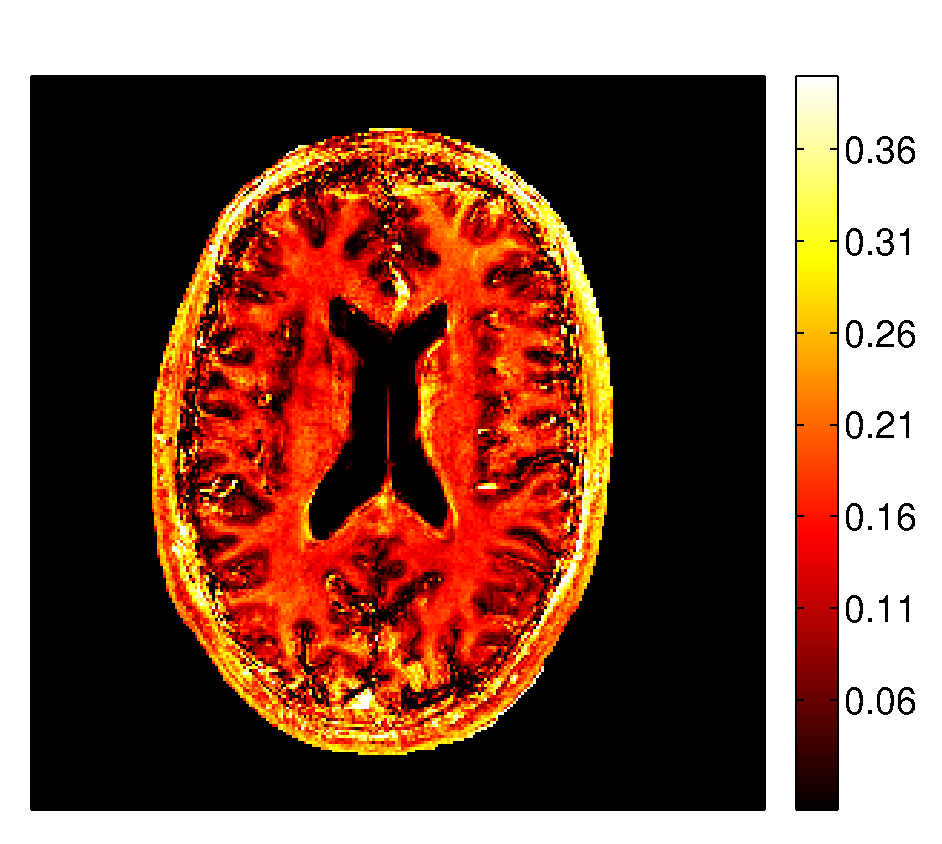
\includegraphics [height=5cm] {%
				c,intro/mwi-ff.eps%
			}%
		\end{minipage}
	\end{figure}
	\vspace{-0.5cm}
	\makebox[3.6cm][r]{qualitative}
	\makebox[6cm][r]{%
		fast-relaxing fraction
		\footnote{%
			figure adapted from \citec{nataraj:17:mwf}
		}%
	}%
\end{frame}

% intro
\begin{frame}{Quantitative MRI (QMRI)}
	\uncover<1->{
		\textbf{Goal}: 
		\hlb{rapidly} and \hlg{accurately} \hlo{localize} \hlm{biomarkers} from MR data
	}
	\begin{itemize}
		\item<2>{
			\makebox[1.8cm][l]{\hlm{biomarker}} measurable tissue property (\eg, flow rate) \\
			\makebox[1.8cm][l]{} that indicates a biological process (\eg, blockage) \\
			\makebox[1.8cm][l]{} characteristic to specific disorders (\eg, stroke)
		}
		\item<3>{\makebox[1.8cm][l]{\hlo{localize}} produce quantitative MR images}
		\item<4>{\makebox[1.8cm][l]{\hlg{accurately}} physically realistic signal models}
		\item<4>{\makebox[1.8cm][l]{\hlb{rapidly}} fast acquisition, fast estimation}
	\end{itemize}
	
	\uncover<5->{
		\textbf{Challenge:} \hlb{rapidly} vs. \hlg{accurately} often competing goals
		\begin{itemize}
			\item{more accurate models typically depend on more markers}
			\item{precisely estimating more markers usually requires \\ longer scans and more computation}
		\end{itemize}
	}
\end{frame}

% overview-acquisition
\begin{frame}{Overview}
	Advances in Quantitative MRI: 
	\begin{itemize}
		\item<1,4>{
			\textbf{Acquisition} \hfill \textcolor{arch-ivy}{[Ch.~4]} \\
			How can we assemble fast, informative collections of scans \\
			to enable precise biomarker quantification? 
		}
		\item<2>{
			\textbf{Estimation} \hfill \textcolor{arch-ivy}{[Ch.~5]} \\
			Given accurate models and informative data, \\
			how can we rapidly quantify these biomarkers?
		}
		\item<3>{
			\textbf{Application} \hfill \textcolor{arch-ivy}{[Ch.~6]} \\
			Using these tools,
			can we design a state-of-the-art biomarker?
		}
	\end{itemize}
\end{frame}

% estimation
% % scan design
\begin{frame}{Signal Model}
	\alt<1>{%
		After reconstruction, 
			single voxel $y_d$ in $d$th image modeled as \\
		\begin{align}
			y_d = s_d\paren{\bmx; \bmnu, \bmp_d} + \epsilon_d
		\end{align}
	}{%
		A \emph{scan profile} is a set of $D$ scans
			that produces at each voxel \\
			a measurement vector $\bmy := \brac{y_1,\dots,y_D}\tpose$ 
			modeled as
			\begin{align}
				\bmy = \bms\paren{\bmx; \bmnu, \bmP} + \bmeps
			\end{align}
	}
	\begin{itemize}
		\item<1>{\makebox[3.5cm][l]{$\bmx \in \reals{L}$} unknown parameters}
		\item<1>{\makebox[3.5cm][l]{$\bmnu \in \reals{K}$} ``known'' parameters}
		\alt<1>{%
			\item<1>{\makebox[3.5cm][l]{$\bmp_d \in \reals{A}$} acquisition parameters}
			\item<1>{\makebox[3.5cm][l]{$s_d : \reals{L+K+A} \mapsto \complex$} 
				$d$th signal model
			}
			\item<1>{\makebox[3.5cm][l]{$\epsilon_d \in \complex$} 
				noise $\sim \cgauss{0}{\sigma_d^2}$
			}
		}{%
			\item<2>{\makebox[3.5cm][l]{$\bmP := \brac{\bmp_1,\dots,\bmp_D}$} 
				acquisition parameter matrix
			}
			\item<2>{\makebox[3.5cm][l]{$\bms : \reals{L+K+AD} \mapsto \complexes{D}$}
				vector signal model
			}
			\item<2>{\makebox[3.5cm][l]{$\bmeps \sim \cgauss{\zeros{D}}{\bmSig}$}
				noise, with $\bmSig := \diag{\sigma_1^2,\dots,\sigma_D^2}$ 
			}
		}
	\end{itemize}
	\uncover<3->{%
		\textbf{Task}: design $\bmP$ to enable precise unbiased estimation of $\bmx$
	}
\end{frame}

\begin{frame}{Towards an Objective Function}
	\uncover<1>{%
  	When $\bms$ is analytic in $\bmx$ (as is typical), \\
  	\textbf{Fisher information} characterizes unbiased estimator precision:
  	\begin{align}
  		\bmF\paren{\bmx; \bmnu, \bmP} := 
  			\paren{\grada{\bmx} \bms\paren{\bmx; \bmnu, \bmP}}\ctpose
  			\bmSig^{-1} \grada{\bmx} \bms\paren{\bmx; \bmnu, \bmP}.
  	\end{align}
  }%
  \uncover<2-4>{%
  	When $\bmF$ is invertible, \Cramer-Rao Bound (CRB) \hfill \citec{cramer:46} \\
  	ensures covariance of unbiased estimates $\est{\bmx}$ of $\bmx$ satisfy
  	\begin{align}
  		\cov{\est{\bmx}; \bmnu, \bmP} \succeq \bmF^{-1}\paren{\bmx; \bmnu, \bmP}.
  	\end{align}
	}%
	\uncover<3>{%
  	Maximum-likelihood (ML) estimates achieve CRB asymptotically \\
  	or equivalently (for Gaussian data) at sufficiently high SNR. \\
	}%
	\uncover<4>{%
		\textbf{Idea}: choose $\bmP$ such that imprecision matrix $\bmF^{-1}$ ``small''
	}
\end{frame}

\begin{frame}{Scan Design}
	\uncover<1-4>{%
		\textbf{Idea}: choose $\bmP$ to minimize the objective 
		\begin{align}
			\costa{\bmx; \bmnu, \bmP} =
        \trace{\bmW \bmF^{-1}\paren{\bmx; \bmnu, \bmP} \bmW\tpose},
		\end{align}
	where $\bmW \in \reals{L\times L}$ is a pre-selected diagonal matrix of weights.
	}%
	\uncover<2>{%
		\textbf{Challenge}: $\bmx,\bmnu$ vary spatially \\
	}
	\uncover<3->{%
  	\textbf{Two problems considered}: 
  	\begin{itemize}
  		\item<3-5>{%
  			min-max scan design \hfill \citec{nataraj:17:oms}
  			\begin{align}
  				\breve{\bmP} &\in \set{
  					\argmin{\bmP \in \setP}
  					\max_{\substack{\bmx \in \setXt \\ \bmnu \in \setNt}}
  					\costa{\bmx; \bmnu, \bmP}
  				}
  			\end{align}
  		}%
			\only<3>{%
				where $\setXt \subseteq \reals{L}$ and $\setNt \subseteq \reals{K}$ 
				are ``tight'' ranges of interest \\
				and $\setP$ is defined by acquisition/timing constraints \\
			}%
  		\item<4>{%
  			Bayesian scan design
  			\begin{align}
  				\breve{\bmP} &\in \set{
  					\argmin{\bmP \in \setP}
  					\expect{\bmx,\bmnu}{\costa{\bmx; \bmnu, \bmP}}
  				}
  			\end{align}
  		}%
  	\end{itemize}
	}
\end{frame}

\begin{frame}{Detailed Example Study}
	\uncover<1->{%
		\textbf{Task}: design fast acquisition for precise estimation 
			of relaxation parameters $\To,\Tt$ in white/gray matter (WM/GM) of brain
	}
	\begin{itemize}
		\item<2>{Consider scan profiles consisting of two fast pulse sequences}
		\begin{itemize}
			\item{Spoiled Gradient-Recalled Echo (SPGR) \hfill \citec{zur:91:sot}}
			\item{Dual-Echo Steady-State (DESS) \hfill \citec{redpath:88:fan}}
		\end{itemize}
		\item<3>{For each scan profile feasible under total time constraint:}
		\begin{enumerate}
			\item{Let $\bms$ model corresponding single-component signal}
			\begin{itemize}
				\item{$\bmx \gets \brac{\mzero, \To, \Tt}\tpose$}, 
					where $\mzero$ is a scale factor
				\item{$\bmnu \gets$ flip angle variation}
				\item{$\bmP \gets$ nominal flip angles, repetition times}
			\end{itemize}
			\item{Optimize $\bmP$ subject to flip angle, sequence timing constraints}
			\begin{itemize}
				\item{$\bmW \gets \diag{0, 0.1, 1}$ emphasizes $\To,\Tt$ est roughly equally}
				\item{$\setXt$ chosen to focus on WM/GM at 3T field strength}
				\item{$\setNt$ chosen to allow 10\% flip angle variation}
			\end{itemize}
		\end{enumerate}
	\end{itemize}
\end{frame}

\begin{frame}{Scan Profile Comparison}
	\uncover<1>{%
  	\begin{table}
      \centering
      {\tabulinesep = 0.5mm
      \begin{tabu} {r | c c c}
         \hline \hline
         (\#SPGR, \#DESS) Profiles & $(2,1)$ & $(1,1)$ & $(0,2)$ \\
         \hline
         SPGR nom. flip (deg) & (15, 5) & 15 & -- \\
         DESS nom. flip (deg) & 30 & 10 & (35, 10) \\
         SPGR rep. times (ms) & (12.2, 12.2) & 13.9 & -- \\
         DESS rep. times (ms) & 17.5 & 28.0 & (24.4, 17.5) \\
         \hline
         \textbf{optimal max cost} & 4.0 & 4.9 & \textbf{3.5} \\
         \hline \hline
  		\end{tabu}}
			\label{table:profile}
  	\end{table}
	}%
	\uncover<2>{%
		\textbf{Main finding}: 
			2 DESS sequences can yield $\To,\Tt$ WM/GM estimates 
			that are at least as precise as $\To,\Tt$ estimates 
			from SPGR/DESS scan profiles, 
			under this competitive time constraint.
	}%
\end{frame}

\begin{comment}
\begin{frame}{Numerical Simulation}
	\uncover<+->{%
		\begin{itemize}
			\item{Simulated many WM-like, GM-like voxel realizations}
			\item{Studied sample statistics of $\To,\Tt$ ML estimates $\ToML,\TtML$}
		\end{itemize}
	}
	\uncover<+->{%
  	\begin{table} [!tb]
      \centering
      {\tabulinesep = 0.2mm
      \begin{tabu} {c | r r r | r}
          \hline \hline
          Profile     & $(2,1)$           & $(1,1)$           & $(0,2)$           & Truth \\
          \hline
          WM $\ToML$  & $830 \pm 17$      & $830 \pm 15$      & $830 \pm 14$      & $832$ \\
          GM $\ToML$  & $1330 \pm 30.$    & $1330 \pm 24$     & $1330 \pm 24$     & $1331$ \\
          \hline
          WM $\TtML$  & $80. \pm 1.0$     & $80. \pm 2.1$     & $79.6 \pm 0.94$   & $79.6$ \\
          GM $\TtML$  & $110. \pm 1.4$    & $110. \pm 3.0$    & $110. \pm 1.6$    & $110$ \\
          \hline \hline
      \end{tabu}}
      \caption{$\ToML,\TtML$ sample means $\pm$ sample standard deviations}
      \label{table:numerical}
  	\end{table}
	}
\end{frame}
\end{comment}

\begin{frame}{Experimental Setup}
	\uncover<1>{%
		Candidate $(2,1)$, $(1,1)$, $(0,2)$ SPGR/DESS scan profiles
		\begin{itemize}
			\item{Prescribed optimized nominal flip angles, repetition times}
			\item{Used $256 \times 256 \times 8$ 3D matrix 
				over $24 \times 24 \times 4$cm FOV}
			\item{Required \textbf{1m37s} scan time for each profile}
		\end{itemize}
	}
	\uncover<2>{%
		Reference scan profile
		\begin{itemize}
			\item{Four inversion recovery (IR) scans for $\To$ estimation}
			\item{Four spin-echo (SE) scans for $\Tt$ estimation}
			\item{$256 \times 256$ matrix over $24 \times 24 \times 0.5$cm FOV}
			\item{Required \textbf{40m58s} scan time total}
		\end{itemize}
	}
	\uncover<3>{%
		Bloch-Siegert (BS) acquisition for separate flip angle calibration
		\begin{itemize}
			\item{Acquired 2 BS-shifted 3D SPGR scans in 1m40s total}
			\item{Used for $\To,\Tt$ est from both candidate and reference profiles}
		\end{itemize}
	}
\end{frame}

\begin{frame}{Phantom Accuracy Results}
	\begin{figure}
		\centering
		\subfloat [$\ToML$ Estimates] {
        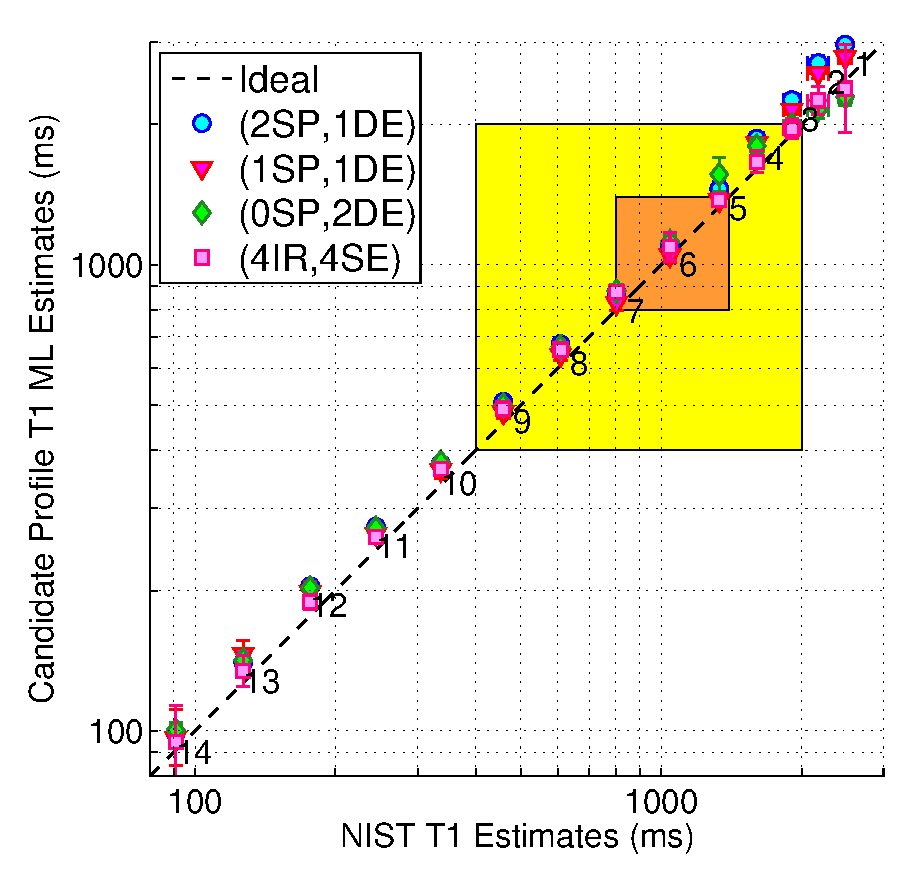
\includegraphics [width = 0.45\textwidth] 
        	{c,scn-dsgn/2016-06-20,hpd,t1-ml-compare.eps}
        \label{fig:scn-dsgn,hpd,t1}
    }
    \hspace{0.3cm}
    \subfloat [$\TtML$ Estimates] {
        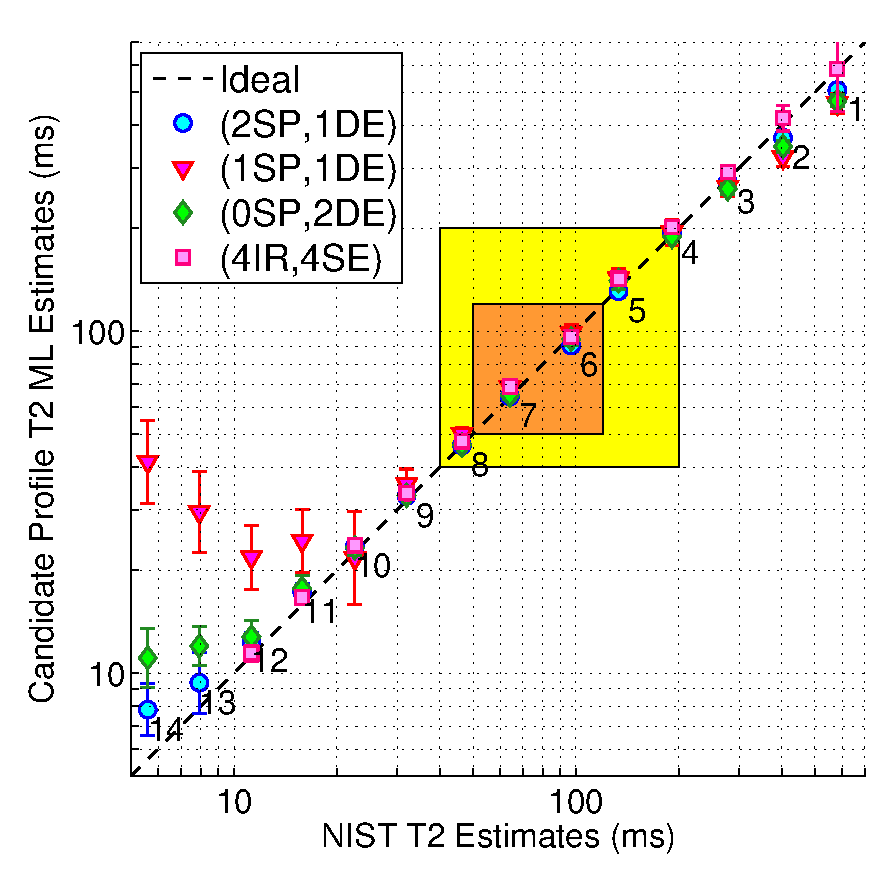
\includegraphics [width = 0.45\textwidth] 
        	{c,scn-dsgn/2016-06-20,hpd,t2-ml-compare.eps}
        \label{fig:scn-dsgn,hpd,t2}
    }
    \label{fig:scn-dsgn,hpd}
 	\end{figure}
	Compared against NIST NMR measurements \hfill \citec{keenan:16:msm}
\end{frame}

\begin{frame}{Phantom Precision Results}
	\only<1>{%
  	\begin{itemize}
  		\item{Repeated each profile 10 times}
  		\item{Estimated $\To,\Tt$ std dev of typical voxel across repetitions}
  	\end{itemize}
	}%
	\uncover<2>{%
  	\begin{table}
      \centering
      \begin{tabu} {c | r r r}
      	\hline \hline
        						    & (2, 1)         		& (1, 1)         		& (0, 2) \\
        \hline
        V5 $\sigToML$   & $50 \pm 12$       & $40 \pm 10.$    	& $39 \pm 9.4$ \\
        V6 $\sigToML$   & $70 \pm 18$       & $60 \pm 15$       & $60 \pm 16$ \\
        V7 $\sigToML$   & $60 \pm 13$       & $50 \pm 13$       & $50 \pm 13$ \\
        \hline 
        V5 $\sigTtML$   & $2.6 \pm 0.63$    & $6 \pm 1.4$       & $3.5 \pm 0.84$ \\
        V6 $\sigTtML$   & $1.9 \pm 0.46$    & $5 \pm 1.1$       & $2.3 \pm 0.54$ \\
        V7 $\sigTtML$   & $1.4 \pm 0.34$    & $3.4 \pm 0.80$    & $1.5 \pm 0.35$ \\
        \hline 
        $\sqrt{\textrm{opt max cost}}$ estimate
        								& $8.9 \pm 1.8$ 		& $11 \pm 2.6$ 			& $\mathbf{8.3 \pm 2.1}$ \\
        \hline \hline
      \end{tabu}
      \caption{
          Pooled sample standard deviations
          $\pm$ pooled standard errors of sample standard deviations (ms),
          from optimized SPGR/DESS profiles.
      }
      \label{table:hpd,sample-std-dev}
  	\end{table}
	}%
	\uncover<3>{%
		Similar trends across profiles of empirical vs. theoretical std dev!
	}
\end{frame}

\begin{frame}{Summary}
	\only<3>{%
		\vspace{-1cm}
  	\begin{figure}
  		\centering
  		\subfloat{
  			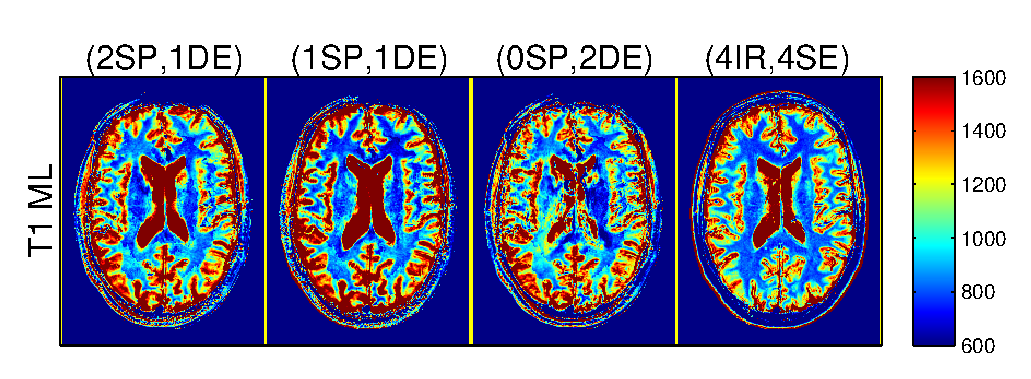
\includegraphics [width=\textwidth, trim=0 0 0 10, clip] 
  				{c,scn-dsgn/2016-05-31,brain,t1-ml,jet.eps}
  			\label{fig:scn-dsgn,brain,t1}
  		}
  		\vspace{0cm}
  		\subfloat{
  			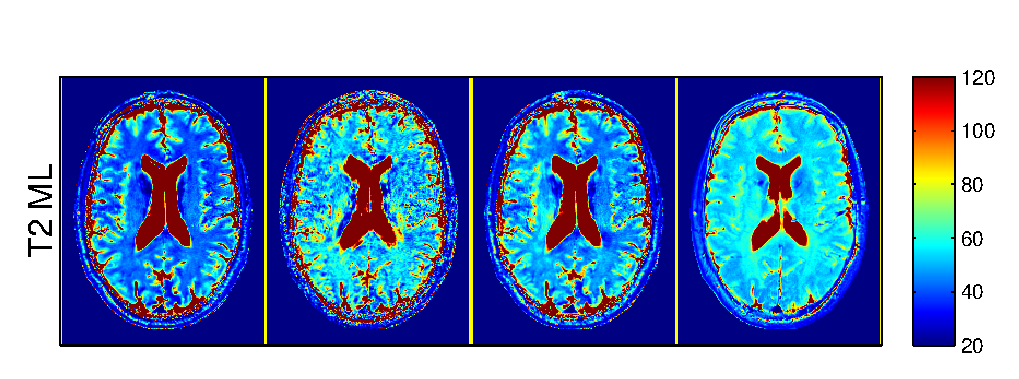
\includegraphics [width=\textwidth-1mm, trim=0 0 0 25, clip]
  				{c,scn-dsgn/2016-05-31,brain,t2-ml,jet.eps}
  			\label{fig:scn-dsgn,brain,t2}
  		}
  		\caption{
  			Colorbar ranges in ms.
  		}
  		\label{fig:scn-dsgn,brain}
  	\end{figure}
	}
	\only<1-2,4-5>{%
  	\uncover<1->{%
  		\textbf{Contributions}
  			\begin{itemize}
  				\item<1->{MR scan design method for precise parameter estimation}
  				\item<1->{Fast SPGR/DESS scan profile for $\To,\Tt$ estimation in brain}
  				\begin{itemize}
  					\item<2->{%
  						Phantom (and omitted simulation) results validate method \\
  						as a predictor of unbiased estimation precision.
  					}
  					\item<4->{
  						\emph{In vivo} results reveal discrepancies 
  						(especially in $\Tt$ estimates),
  						suggesting $\To,\Tt$ estimates sensitive to model mismatch.
  					}
  				\end{itemize}
  			\end{itemize}
  	}
  	\uncover<5>{%
  		\textbf{How to address \invivo model mismatch?}
  		\begin{itemize}	
  			\item{More accurate \invivo signal models}
  			\item{More scalable parameter estimation}
  		\end{itemize}
  	}
	}
\end{frame}


% overview-estimation
\begin{frame}{Overview}
	Advances in Quantitative MRI: 
	\begin{itemize}
		\item<0>{
			\textbf{Acquisition} \hfill \textcolor{arch-ivy}{[Ch.~4]} \\
			How can we assemble fast, informative collections of scans \\
			to enable precise biomarker quantification? 
		}
		\item<1>{
			\textbf{Estimation} \hfill \textcolor{arch-ivy}{[Ch.~5]} \\
			Given accurate models and informative data, \\
			how can we rapidly quantify these biomarkers?
		}
		\item<0>{
			\textbf{Application} \hfill \textcolor{arch-ivy}{[Ch.~6]} \\
			Using these tools,
			can we design a state-of-the-art biomarker?
		}
	\end{itemize}
\end{frame}

% estimation
% perk
\begin{frame}{Signal Model}
	\uncover<+->{%
		\textbf{Given}: at every voxel, measurement vector $\bmy \in \complexes{D}$ modeled as 
		\begin{align}
			\bmy = \bms\paren{\bmx,\bmnu} + \bmeps
			\label{eq:model}
		\end{align}
		\begin{itemize}
			\item{\makebox[3cm][l]{$\bmx \in \reals{L}$} unknown parameters}
			\item{\makebox[3cm][l]{$\bmnu \in \reals{K}$} ``known'' parameters}
			\item{\makebox[3cm][l]{$\bms : \reals{L+K} \mapsto \complexes{D}$} 
				vector signal model}
			\item{%
				\makebox[3cm][l]{$\bmeps \in \complexes{D}$} 
				noise $\sim \cgauss{\zeros{D}}{\bmSig}$
			}%
		\end{itemize}
		\vspace{0.5cm}
	}%
	\uncover<+->{%
		\textbf{Task}: design fast voxel-by-voxel estimator $\esta{\bmx}{\bmy,\bmnu}$
	}%
\end{frame}

\begin{frame}{Prior Work}
	\uncover<1->{%
		\textbf{Task}: design fast voxel-by-voxel estimator $\esta{\bmx}{\bmy,\bmnu}$
  	
  	\textbf{Challenges}:
  	\begin{itemize}
  		\item{signal $\bms$ often nonlinear in $\bmx$: non-convex inverse problems}
  		\item{signal $\bms$ might be difficult to write in closed form}
  	\end{itemize}
	}%
	\uncover<2->{%
  	\textbf{Conventional Approaches:}
	}%
  	\begin{itemize}
			\item<2-3>{gradient-based local optimization}
			\begin{itemize}
				\item{initialization-dependent solution}
				\item{requires signal gradients}
			\end{itemize}
  		\item<3>{stochastic methods (\eg, simulated annealing)}
  		\begin{itemize}
  			\item{unclear convergence analysis \hfill \citec{bertsimas:93:sa}}
  			\item{several unintuitive tuning parameters}
  		\end{itemize}
			\item<4>{%
				dictionary-based grid search
			}%
  	\end{itemize}
\end{frame}

\begin{frame}{Motivation}
	\textbf{Grid search} computational costs
	\begin{table}
		\centering
		\begin{tabular}{r|cc}
			& $L$ & $\sim$number dictionary atoms \\
			\hline
			\uncover<1-2>{1-compartment relaxivity 		& 3 		& $\sim$$100^2$ \\}
			\uncover<2>{flow velocity 									& 4 		& $\sim$$100^3$ \\} 
			\uncover<2>{diffusivity tensor 							& 7 		& $\sim$$100^6$ \\}
			\uncover<2->{\hlg{2-3 compartment relaxivity}& 6-10 	& $\sim$$100^5-100^9$} 
			\end{tabular}
		\end{table}
		
		\uncover<3>{
			\textbf{Can we scale computation with $L$ more gracefully?}
		}
\end{frame}

\begin{frame}{Machine Learning for QMRI Parameter Estimation}
	\uncover<1->{%
		\textbf{Idea}: learn a \emph{nonlinear} estimator from simulated training data
	}
	\begin{itemize}
		\item<2-3>{%
			sample $\paren{\bmx_1,\bmnu_1,\bmeps_1},\dots,\paren{\bmx_N,\bmnu_N,\bmeps_N}$
			from prior distributions
		}
		\item<2-3>{%
			simulate image data vectors $\bmy_1,\dots,\bmy_N$ 
			via signal model $\bms$
		}
		\item<3-5>{%
			design \emph{nonlinear} functions 
				$\est{x}_l\paren{\cdot} := \est{h}_l\paren{\cdot} + \est{b}_l$ 
				for $l \in \set{1,\dots,L}$ \\
				that map each 
				$\bmq_n := [\re{\bmy_n}\tpose, \im{\bmy_n}\tpose, \bmnu_n\tpose]\tpose \in \setQ$	
				to $x_{l,n} \in \real$
		}
	\end{itemize}	
	\vspace{-0.3cm}
	\uncover<4->{%
		\alt<4-5>{%
			\begin{align}
				\paren{\est{h}_l,\est{b}_l} \in \set{
					\argmin{\substack{h_l \\ b_l \in \real}} 
					\frac{1}{N} \sum_{n=1}^N \paren{h_l\paren{\bmq_n} + b_l - x_{l,n}}^2
				}%
				\uncover<5>{%
					\,\,\,\,\, \textcolor{red}{\text{ill-posed!}}
				}%
				\nonumber
			\end{align}
		}{%
			\begin{align}
				\paren{\est{h}_l,\est{b}_l} \in \set{%
					\argmin{\substack{h_l \hlb{\in \hilb} \\ b_l \in \real}}
					\frac{1}{N} \sum_{n=1}^N \paren{h_l\paren{\bmq_n} + b_l - x_{l,n}}^2
					\hlb{+ \rho_l \norm{h_l}^2_\hilb}
				}%
				\label{eq:krr,cost}
			\end{align}
		}%
	}%
	\uncover<6->{%
		\textbf{Solution}: Param Estimation via Regression with \hlm{Kernels} (PERK) \\
			\hfill \citec{nataraj::dfm}%
		\begin{itemize}
			\item{restrict optimization to a \hlb{certain rich function space $\hilb$}}
			\item{optimal $\est{h}_l \hlb{\in \hilb}$ takes form 
				$\est{h}_l = \sum_{n=1}^N \est{a}_{l,n} \hlm{k}(\cdot,\bmq_n)$ \\
				\hfill \citec{scholkopf:01:agr}}
		\end{itemize}
	}	
\end{frame}

\begin{frame}{PERK in a 1-D Toy Problem}
	\uncover<1->{%
		\textbf{Task}: 
			estimate $\Tt$, given samples from $y = \exp\paren{-\TE/\Tt} + \epsilon$
		\vspace{-0.5cm}
		\begin{figure}
			\subfloat[$N\gets10$]{%
				\includegraphics [width=0.33\textwidth] {%
					c,perk/toy/toy-1d,t2-se,n-10%
				}%
			}%
			\subfloat[$N\gets20$]{%
				\includegraphics [width=0.33\textwidth] {%
					c,perk/toy/toy-1d,t2-se,n-20%
				}%
			}%
			\subfloat[$N\gets50$]{%
				\includegraphics [width=0.33\textwidth] {%
					c,perk/toy/toy-1d,t2-se,n-50%
				}%
			}%
		\end{figure}
	}%
	\uncover<1->{%
		\textbf{Compare}: $\TtPERK$ with method-of-moments (MOM) estimator 
			$$\TtMOM\paren{\cdot} := -\TE/\log{\abs{\cdot}}$$
		(PERK more useful when good MOM estimator unavailable)
	}%
\end{frame}

\begin{frame}{PERK Solution}
	Non-iterative closed-form solution, for $l \in \set{1,\dots,L}$: 
	\begin{align}
		\est{x}_l\paren{\cdot} = \bmxg{l}\tpose\paren{
			\frac{1}{N}\ones{N} 
			+ \bmM\inv{\bmK\bmM + N\rho_l \eye{N}} 
			\paren{\bmka{\cdot} - \frac{1}{N}\bmK\ones{N}}
		}
		\label{eq:krr,x-hat}
	\end{align}
	\begin{itemize}
	\item<1-4>{%
		\makebox[6cm][l]{$\bmxg{l} := [x_{l,1},\dots,x_{l,N}]\tpose$}
		training pt regressands
	}
	\item<2-4,6>{%
		\makebox[6cm][l]{%
			$\bmK := 
				\begin{bmatrix}
					\hlm{k}(\bmq_1,\bmq_1) 	& \cdots 	& \hlm{k}(\bmq_1,\bmq_N) \\
					\vdots									& \ddots	& \vdots \\
					\hlm{k}(\bmq_N,\bmq_1) 	& \cdots 	& \hlm{k}(\bmq_N,\bmq_N)
				\end{bmatrix}$
		}
		Gram matrix
	}						
	\item<3-4>{%
		\makebox[6cm][l]{$\bmM := \eye{N} - \frac{1}{N}\ones{N}\ones{N}\tpose$}
		de-meaning operator
	}
	\item<4>{%
		\makebox[6cm][l]{%
			$\bmka{\cdot} := \brac{\hlm{k}(\cdot,\bmq_1),\dots,\hlm{k}(\cdot,\bmq_N)}\tpose$
		}
		nonlin kernel embedding
	}
	\end{itemize}
	\uncover<5>{%
		Can we scale computation with $L$ more gracefully?
	}
	\begin{itemize}
		\item<5>{Perhaps, since \eqref{eq:krr,x-hat} separable in $l \in \set{1,\dots,L}$ by construction}
		\item<6>{However, explicitly computing $\bmK$ may be undesirable...}
	\end{itemize}
\end{frame}

\begin{frame}{PERK as High-Dimensional Affine Regression}
	\uncover<1->{
		Suppose there exists``approximate feature mapping'' $\bmztZ : \setQ \mapsto \reals{Z}$ \\
		such that $\bmZt := \brac{\bmztZa{\bmq_1},\dots,\bmztZa{\bmq_N}}$ has for $\dim\paren{\setQ} \ll Z \ll N$
		\begin{align}
			\bmK \approx \bmZt\tpose \bmZt.
			\label{eq:low-rank}
		\end{align}
		\vspace{-0.5cm}
	}
	\uncover<2-3>{%
		\begin{overlayarea}{\textwidth}{2.5cm}
  		\alt<2>{%
    		Plugging \eqref{eq:low-rank} into PERK solution \eqref{eq:krr,x-hat} and rearranging gives
    		\begin{align}
    			\est{x}_l\paren{\cdot} \approx 
    				\frac{1}{N}\bmxg{l}\tpose\ones{N} 
    				+ \frac{1}{N}\bmxg{l}\tpose \bmM \bmZt\tpose
    				\inv{\frac{1}{N} \bmZt \bmM \bmZt\tpose + \rho_l\eye{Z}}
    				\paren{\bmztZa{\cdot}-\frac{1}{N}\bmZt\ones{N}}
    				\nonumber
    		\end{align}
    	}{%
    		Plugging \eqref{eq:low-rank} into PERK solution \eqref{eq:krr,x-hat} and rearranging gives
    		\begin{align}
    			\est{x}_l\paren{\cdot} \approx 
    				\mxl + \cxlzt \inv{\Cztzt + \rho_l\eye{Z}} \paren{\bmztZa{\cdot} - \bmmzt}
    				\label{eq:x-cme}
    		\end{align}
				which is regularized $Z$-dimensional affine regression!
    	}
		\end{overlayarea}
	}
	\uncover<4->{%
		Does such a $\bmzt$ exist and work well in practice?
		\begin{itemize}
			\item{Yes, \eg for Gaussian
				$\hlm{k}(\bmq,\bmq') \gets \expa{-\frac{1}{2}\norm{\bmL^{-1}\paren{\bmq-\bmq'}}_2^2}$ \\
				\hfill \citec{rahimi:07:rff}}
			\item{In such cases, can reduce from $\sim$$N^2$ to $\sim$$NZ$ computations}
		\end{itemize}
	}
\end{frame}

\begin{frame}{Experimental Setup}
	\uncover<1->{%
		Demonstrated PERK for $\To,\Tt$ est from optim (2SP,1DE) scan
	}%
	\begin{itemize}
		\item<2>{%
			PERK trained using $N \gets 10^5$ samples from prior dist $\dist{\bmx,\bmnu}$
		}%
		\item<2>{%
			To enable precise estimation,
			support of $\dist{\bmx,\bmnu}$ carefully chosen \\
			to coincide with min-max acquisition design support
		}%
	\end{itemize}
	
	\uncover<3->{%
		Compared PERK to two well-suited ML estimators:
		\begin{itemize}
			\item{%
				dictionary-based grid search estimator via \\
				variable projection method (VPM) \hfill \citec{golub:03:snl}
			}%
			\item{%
				local optim estimator via preconditioned variant (PGPM) \\
				of classical gradient projection method \hfill \citec{rosen:60:tgp}
			}%
		\end{itemize}
	}%
\end{frame}
	
\begin{frame}{Phantom Results}
	\vspace{-0.3cm}
	\uncover<1->{%
  	\begin{figure}
			\centering
			\begin{minipage}{0.7\textwidth}
  			\subfloat{%
  				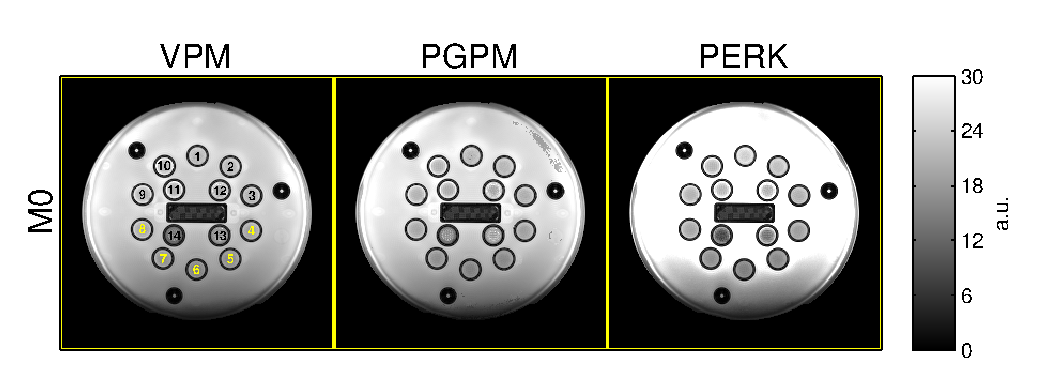
\includegraphics [width=0.96\textwidth,clip] {%
  					c,perk/hpd-tight/sp2de1,sl-6,m0,im-gray.eps%
  				}%
  			}%
  			\hspace{0cm}
    		\subfloat{%
  				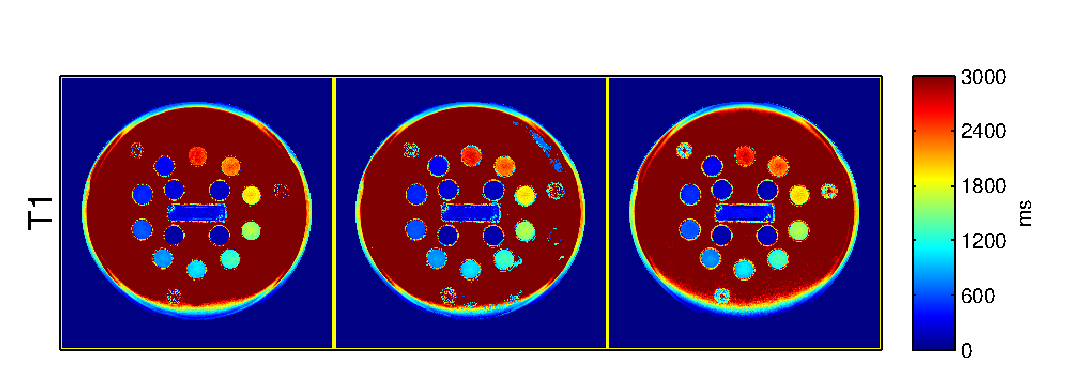
\includegraphics [width=0.982\textwidth,trim=0 0 0 25,clip] {%
  					c,perk/hpd-tight/sp2de1,sl-6,t1,im-jet.eps%
  				}%
  			}%
  			\hspace{0cm}
    		\subfloat{%
  				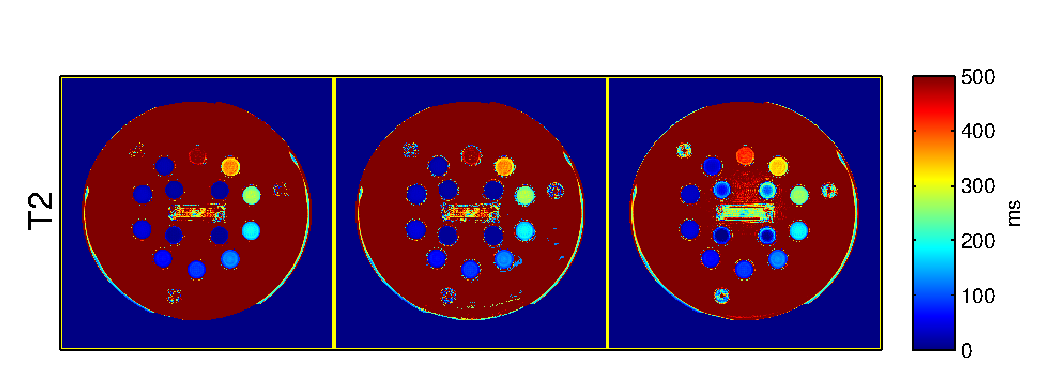
\includegraphics [width=0.97\textwidth,trim=0 0 0 25,clip] {%
  					c,perk/hpd-tight/sp2de1,sl-6,t2,im-jet.eps%
  				}%
  			}%
			\end{minipage}
			\label{fig:perk,hpd-tight,im}
  	\end{figure}
	}%
	\vspace{-0.3cm}
	\uncover<2->{%
		\makebox[3.3cm][r]{$928$s}
		\makebox[1.9cm][r]{$1257$s}
		\makebox[2.1cm][r]{$4.2$s train} \\
		\vspace{-0.1cm}
		\makebox[7.4cm][r]{$1.9$s test}
	}	
\end{frame}
	
\begin{frame}{Phantom Results}
	\uncover<1->{%
  	\begin{figure}
  		\centering
  		\subfloat{%
				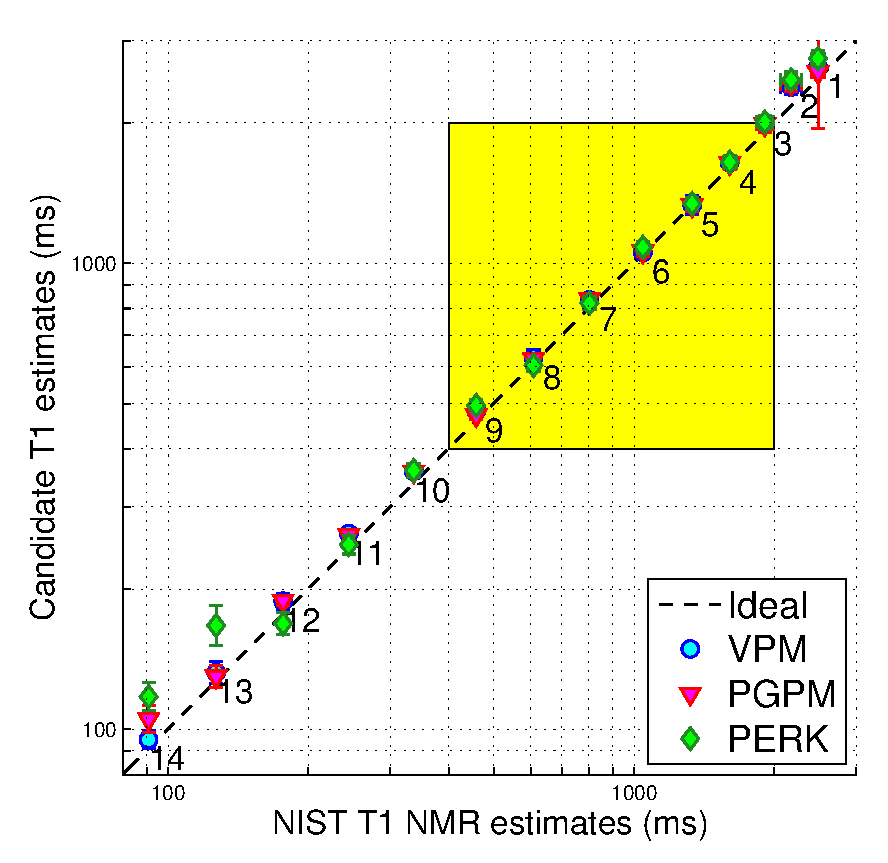
\includegraphics [width=0.45\textwidth] 
          {c,perk/hpd-tight/sp2de1,sl-6,t1,plot.eps}
        \label{fig:perk,hpd,plot,t1}
      }%
      \hspace{0.3cm}
      \subfloat{%
      	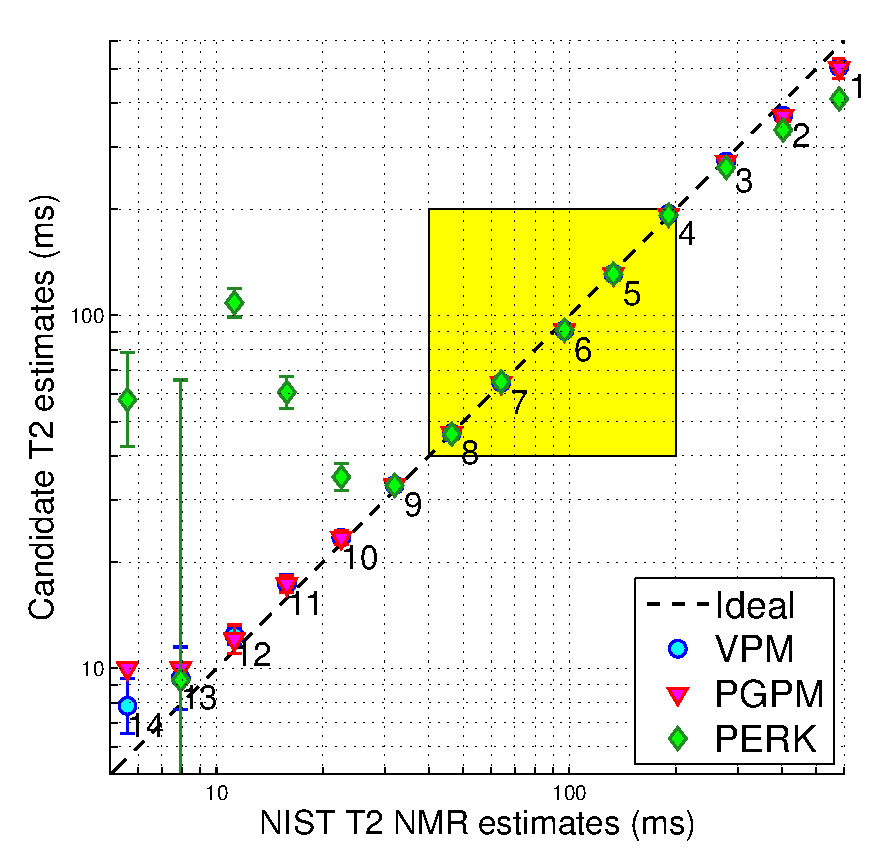
\includegraphics [width=0.45\textwidth] 
					{c,perk/hpd-tight/sp2de1,sl-6,t2,plot.eps}
				\label{fig:perk,hpd,plot,t2}
      }%
      \label{fig:perk,hpd-tight,plot}
   	\end{figure}
	}%
	\uncover<2->{%
		Within support of $\dist{\bmx,\bmnu}$, \\
		\textbf{PERK and grid search estimates agree excellently}.
	}%
\end{frame}

\begin{frame}{\emph{In vivo} Results}
	\vspace{-0.3cm}
	\uncover<1->{%
  	\begin{figure}
			\centering
			\begin{minipage}{0.6\textwidth}
  			\subfloat{%
  				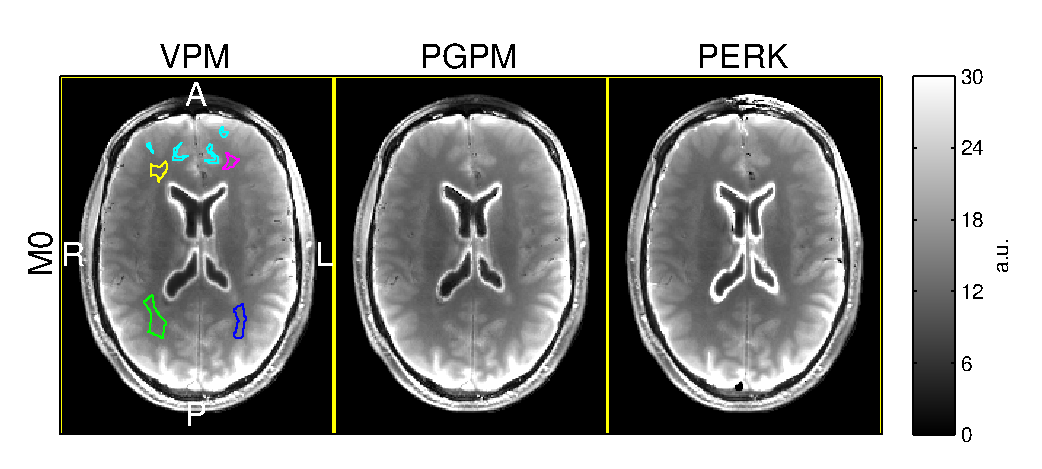
\includegraphics [width=0.96\textwidth,trim=0 0 0 10,clip] {%
  					c,perk/brain/sp2de1,sl-5,m0,im-gray.eps%
  				}%
  			}%
  			\hspace{0cm}
    		\subfloat{%
  				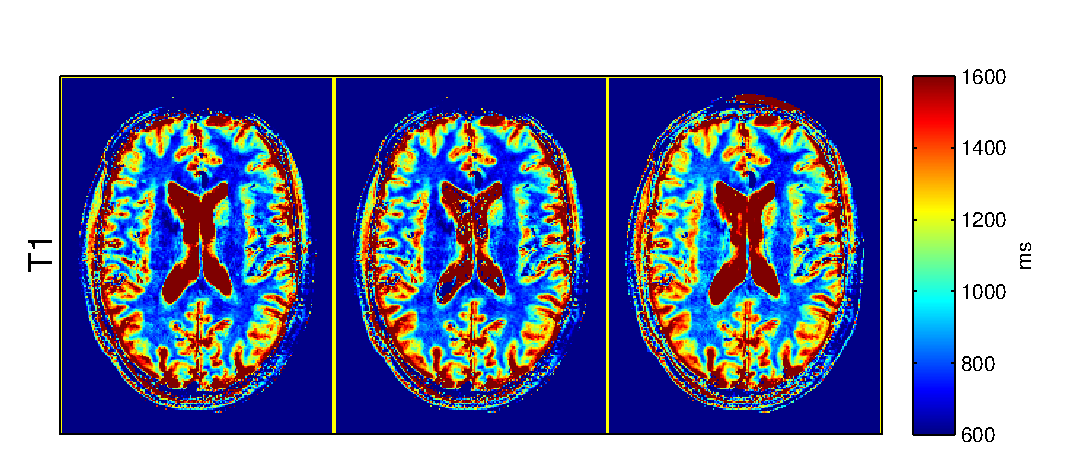
\includegraphics [width=0.982\textwidth,trim=0 0 0 20,clip] {%
  					c,perk/brain/sp2de1,sl-5,t1,im-jet.eps%
  				}%
  			}%
  			\hspace{0cm}
    		\subfloat{%
  				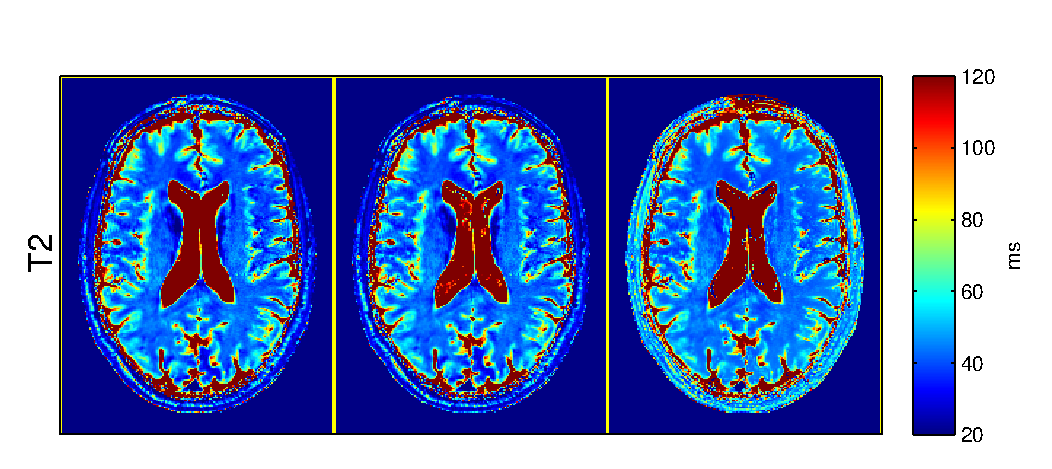
\includegraphics [width=0.97\textwidth,trim=0 0 0 20,clip] {%
  					c,perk/brain/sp2de1,sl-5,t2,im-jet.eps%
  				}%
  			}%
			\end{minipage}
			\label{fig:perk,hpd-tight}
  	\end{figure}
	}%
	\vspace{-0.3cm}
	\uncover<2->{%
		\makebox[3.6cm][r]{$838$s}
		\makebox[1.65cm][r]{$2178$s}
		\makebox[1.9cm][r]{$4.2$s train} \\
		\vspace{-0.1cm}
		\makebox[7.3cm][r]{$1.6$s test}
	}
\end{frame}

\begin{frame}{Summary}
	\uncover<1->{%
		\textbf{Contributions}
		\begin{itemize}
			\item<1->{\textbf{PERK}: fast, dictionary-free estimator for QMRI}
			\item<2->{demonstrated PERK for $\To,\Tt$ estimation}
			\begin{itemize}
				\item<2>{%
					Phantom (and omitted simulation) results show that \\
					PERK and ML estimators yield comparable accuracy/precision
				}
				\item<2>{%
					\emph{In vivo} PERK and ML estimates are comparable in WM/GM
				}
				\item<2-3>{%
					\textbf{PERK is consistently at least $140$x faster}
				}
			\end{itemize}
		\end{itemize}
	}
	\uncover<3>{%
		\textbf{Can we exploit PERK's speed in a more compelling problem?}
	}
\end{frame}


% overview-application
\begin{frame}{Overview}
	Advances in Quantitative MRI: 
	\begin{itemize}
		\item<0>{
			\textbf{Acquisition} \hfill \textcolor{arch-ivy}{[Ch.~4]} \\
			How can we assemble fast, informative collections of scans \\
			to enable precise biomarker quantification? 
		}
		\item<0>{
			\textbf{Estimation} \hfill \textcolor{arch-ivy}{[Ch.~5]} \\
			Given accurate models and informative data, \\
			how can we rapidly quantify these biomarkers?
		}
		\item<1>{
			\textbf{Application} \hfill \textcolor{arch-ivy}{[Ch.~6]} \\
			Using these tools,
			can we design a state-of-the-art biomarker?
		}
	\end{itemize}
\end{frame}

% application
% % myelin water fraction imaging
\begin{frame}{Background}
	\begin{minipage}{0.6\textwidth}
		\uncover<2-3>{%
			Myelin water fraction (MWF): 
  		\begin{itemize}
  			\item<2->{%
  				Proportion of MR signal arising 
  				from water trapped within myelin bilayers,
  				relative to total signal \hfill \citec{mackay:94:ivv}
  			}
  			\item<3->{%
  				Correlates well with myelin content \hfill \citec{webb:03:imt}
  			}
  		\end{itemize}
		}
	\end{minipage}
	\begin{minipage}{0.36\textwidth}
		\uncover<1-3>{%
			\begin{figure}
				\centering
				\includegraphics[width=3.5cm]{c,mwf/myelin}
			\end{figure}
			\hfill www.mayoclinic.org
		}
	\end{minipage}
\end{frame}

\begin{frame}{Previous MWF imaging acquisitions}
	\uncover<1>{%
  	Multi-echo spin-echo (\textbf{MESE}) \hfill \citec{mackay:94:ivv}
  	\begin{itemize}
  		\item{Gold-standard}
  		\item{Speed-limited by long repetition times ($\sim$2s)}
  	\end{itemize}
  }
  \uncover<2>{%
  	Combinations of fast steady-state scans using variable flip angles (``\textbf{mcDESPOT}'') 
  		\hfill \citec{deoni:08:gmt}
  	\begin{itemize}
  		\item{Whole-brain, high-resolution MWF imaging in $\sim$30m}
  		\item{%
  			Disagree with MESE MWF estimates, \hfill \citec{zhang:15:com}
  			likely due to insufficient precision \hfill \citec{lankford:13:oti}
  		}
  	\end{itemize}
	}
	\uncover<3->{%
		\textbf{Goal}: fast, precise MWF quantification in WM
	}
\end{frame}

\begin{frame}{A voxel-scale MWF model}
	\begin{figure}
		\begin{tikzpicture}
			\uncover<1->{
				\node[above] at (2,4) {simple two-compartment model};
				\draw[thick,fill=gray!10] (0,0) -- (2,0) -- (1,4) -- (0,4) -- (0,0);
				\draw[thick,fill=gray!30] (2,0) -- (4,0) -- (4,4) -- (1,4);
				\node[below] at (1,0) {``fast''};
				\node[below] at (3,0) {``slow''};
			}
			\only<2-3>{
				\node[below right] at (0,0.7) {$\tf{1},\tf{2}$};
				\node[below left] at (4,0.7) {$\ts{1},\ts{2}$};
  			\alt<2>{
  				\node at (2.7,2) {$\paren{1-\ff}\mzero$};
  				\node at (0.7,2) {$\ff \mzero$};
  			}{
  				\node at (2.7,2) {$\paren{1-\hlg{\ff}}\mzero$};
  				\node at (0.7,2) {$\hlg{\ff} \mzero$};
  			}
			}
		\end{tikzpicture}
	\end{figure}
	\uncover<3->{
		Take fast-relaxing fraction $\hlg{\ff}$ as a simple proxy for MWF
	}
\end{frame}

\begin{frame}{Multi-compartmental MR signal models}
	\uncover<1-3>{%
		2-compartment SPGR model \hfill \citec{spencer:00:mos} \\
	}
	\begin{itemize}
		\item<1>{included first-order physical exchange}
		\item<2,5>{neglected relaxation, precession, exchange during excitation}
		\item<3,5>{%
			absorbing off-resonance effects into $\mzero$ 
			\emph{implies} neglecting exchange between excitation and readout
		}
	\end{itemize}
	\uncover<4->{%
		Two-compartment DESS model \hfill \textcolor{arch-ivy}{[\S6.2.2]}%
	}
	\begin{itemize}
		\item<4-5>{%
			additional approximations required 
			unless we assume time-independent diff 
			in compartmental off-resonance freq
		}
		\item<5>{%
			including exchange, closed-form solutions still elusive
		}
	\end{itemize}
	\uncover<6>{%
		\textbf{For simplicity, we neglect exchange.}
	}
\end{frame}

\begin{frame}{Bayesian MWF Scan Design}
	\begin{align}
    \breve{\bmP} &\in 
    	\set{
        \argmin{\bmP \in \setP}
        \expcost\paren{\bmP}
    	}, \where \nonumber \\
		\expcost\paren{\bmP} &:=
    	\expect{\bmx,\bmnu}{\trace{\bmW \bmF^{-1}\paren{\bmx; \bmnu, \bmP} \bmW\tpose}}
  \end{align}
  \vspace{-0.5cm}
  \begin{itemize}
  	\item<2>{%
			\makebox[1.5cm][l]{$\bmx$} 
			$\brac{\hlg{\ff}, \tf{1}, \tf{2}, \ts{1}, \ts{2}, \mzero}\tpose$
		}
		\item<2>{%
			\makebox[1.5cm][l]{$\bmnu$}
			flip angle variation
		}
		\item<2>{%
			\makebox[1.5cm][l]{$\bmP$}
			SPGR/DESS nominal flip angles, repetition times
		}
		\item<3>{%
			\makebox[1.5cm][l]{$\bmW$}
			$\diag{\brac{\inv{\expect{\bmx,\bmnu}{\hlg{\ff}}}, \zeros{5}\tpose}\tpose}$
		}
		\item<4>{%
			\makebox[1.5cm][l]{$\expect{\bmx,\bmnu}{\cdot}$}
			approximated via empirical averages \\
			\makebox[1.5cm][l]{}
			of samples drawn from separable prior
		}
		\item<5>{%
			\makebox[1.5cm][l]{$\setP$}
			nom flip angle, total scan time constraints
		}
  \end{itemize}
\end{frame}

\begin{frame}{Optimized SPGR/DESS Acquisition}
	\begin{table}[!tb]
    \centering
    \begin{tabular}{r | c | c}
      \hline
      \hline
      & Optimized flip angles (deg) & Optimized rep. times (ms) \\
      \hline
      SPGR & $38.1,12.9,9.2,33.5$ 	& $50.2,32.4,16.4,11.8$ \\
      DESS & $32.0,40.3,52.9$ 			& $17.5,98.0,37.6$ \\
      \hline
      \hline
    \end{tabular}
    \caption{Optimized Scan Parameters, $\breve{\bmP}$}
		\label{tab:mwf,acq}
	\end{table}
	\begin{itemize}
		\item{%
			Predicted MWF relative standard deviation in WM
			\begin{itemize} 
				\item{%
					Optimized SPGR/DESS:
					$\sqrt{\expcost\paren{\breve{\bmP}}} = 0.285$
				}
				\item{%
					mcDESPOT: at least $1$ \hfill \citec{lankford:13:oti}
				}
			\end{itemize}
		} 
	\end{itemize}
\end{frame}

\begin{frame}{MWF Estimation via KRR}
	\uncover<1>{%
		\textbf{Simulation Setup}
		\begin{itemize}
			\item{At each voxel, generate ground-truth $\bmx,\bmnu$}
			\item{Using 2-compartment SPGR/DESS model $\bms$
				with optimized (and now fixed) parameters $\breve{\bmP}$,
				generate voxel data $\bmy \in \complexes{10}$
			}
		\end{itemize}
	}
	\uncover<2>{%
		\textbf{Use KRR to estimate just $\hlg{\ff}$}
		\begin{itemize}
			\item{Separable prior on $\bmx$: $\hlg{\ff},\mzero$ uniform; others log-uniform}
			\item{$N \gets 10^6$ training points}
			\item{$Z \gets 10^3$ kernel approximation order}
		\end{itemize}
	}
	\uncover<3>{%
		\textbf{Compare against grid search}
		\begin{itemize}
			\item{unconstrained search would require $\sim$100$^{5}$ dictionary atoms}
			\item{we artificially constrain search here to limit computation}
		\end{itemize}
	}
\end{frame}

\begin{frame}{MWF Simulation Result}
	Fast-fraction $\hlg{\ff}$ estimates, in simulation: 
	\uncover<+->{%
		\begin{figure}[t]
			\centering
			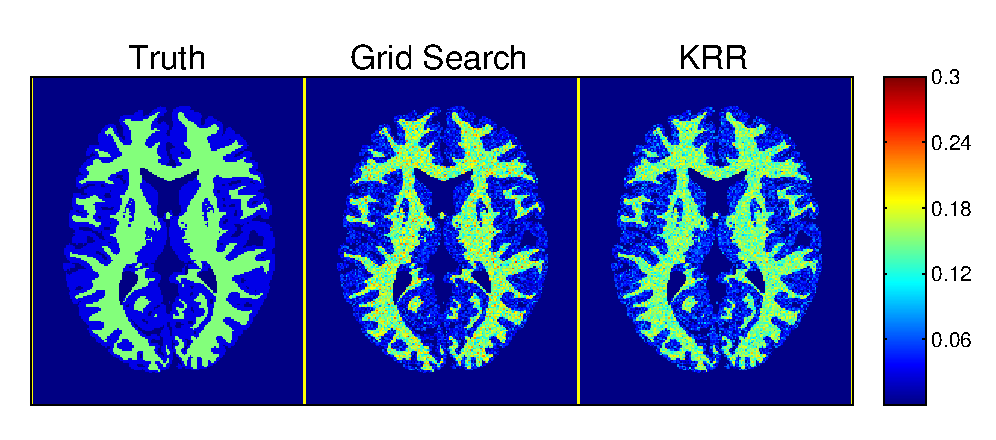
\includegraphics[width=\textwidth]{c,krr/sim-talk}%
		\end{figure}
	}
	\uncover<+->{%
		\makebox[5cm][r]{$\sim$4h}
		\makebox[4.7cm][r]{$40$s training, $2$s testing}
	}	
\end{frame}

\begin{frame}{MWF Proof-of-concept Experimental Study}
	\uncover<1>{%
		Acquired \invivo data using optimized MWF protocol
		\begin{itemize}
			\item{Used $256\times256\times8$ 3D matrix over $24\times24\times4$cm FOV}
			\item{Required \textbf{11m48s} total (including BS scan)} 
		\end{itemize} 
	}
	\uncover<2-4>{%
		Rapidly estimated $\hlg{\ff}$ as proxy for MWF
		\begin{itemize}
			\item<2>{Full-scale grid search intractable on typical desktop}
			\item<3-4>{KRR training and testing took \textbf{35s} and \textbf{5s/slice}}
			\item<4>{Iterative ML refinement took \textbf{29s/slice}}
		\end{itemize}
	}
	\uncover<5->{%
		Compared (qualitatively) with results in \hfill \citec{zhang:15:com}%
		\begin{itemize}
			\item{GRASE: accelerated MESE acq \hfill \citec{prasloski:12:rwc}}
			\item{mcDESPOT: 9 SPGR, 18 bSSFP scans \hfill \citec{deoni:11:com}}
		\end{itemize}	
	}
\end{frame}

\begin{frame}{MWF Proof-of-concept In Vivo Result}
	\vspace{-0.3cm}
	\begin{figure}
    \centering
    \begin{minipage}[b]{0.7\textwidth}
        \centering
        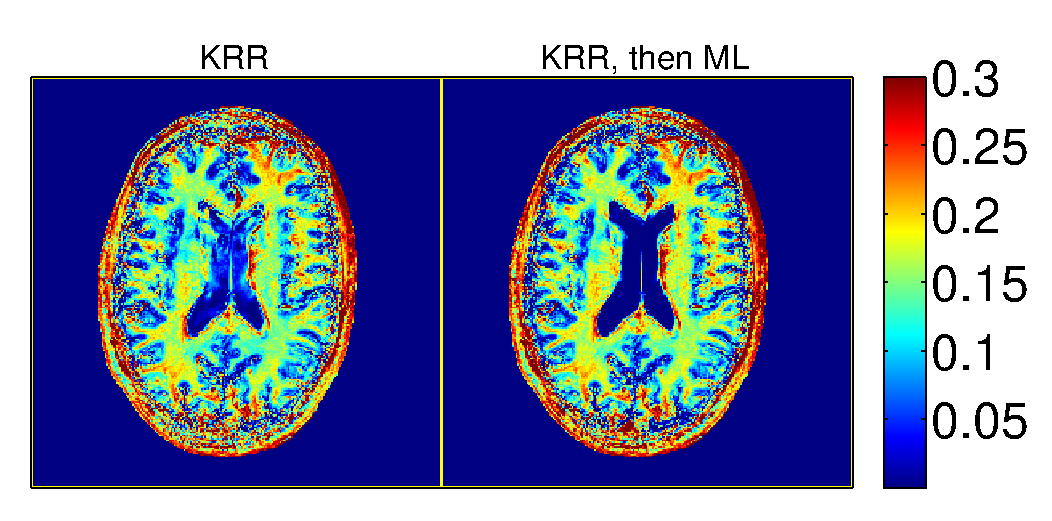
\includegraphics [height=4cm, clip] {c,mwf/ff,log2c-0,krr-ml}
    \end{minipage}

    \begin{minipage}[b]{0.96\textwidth}
        \centering
        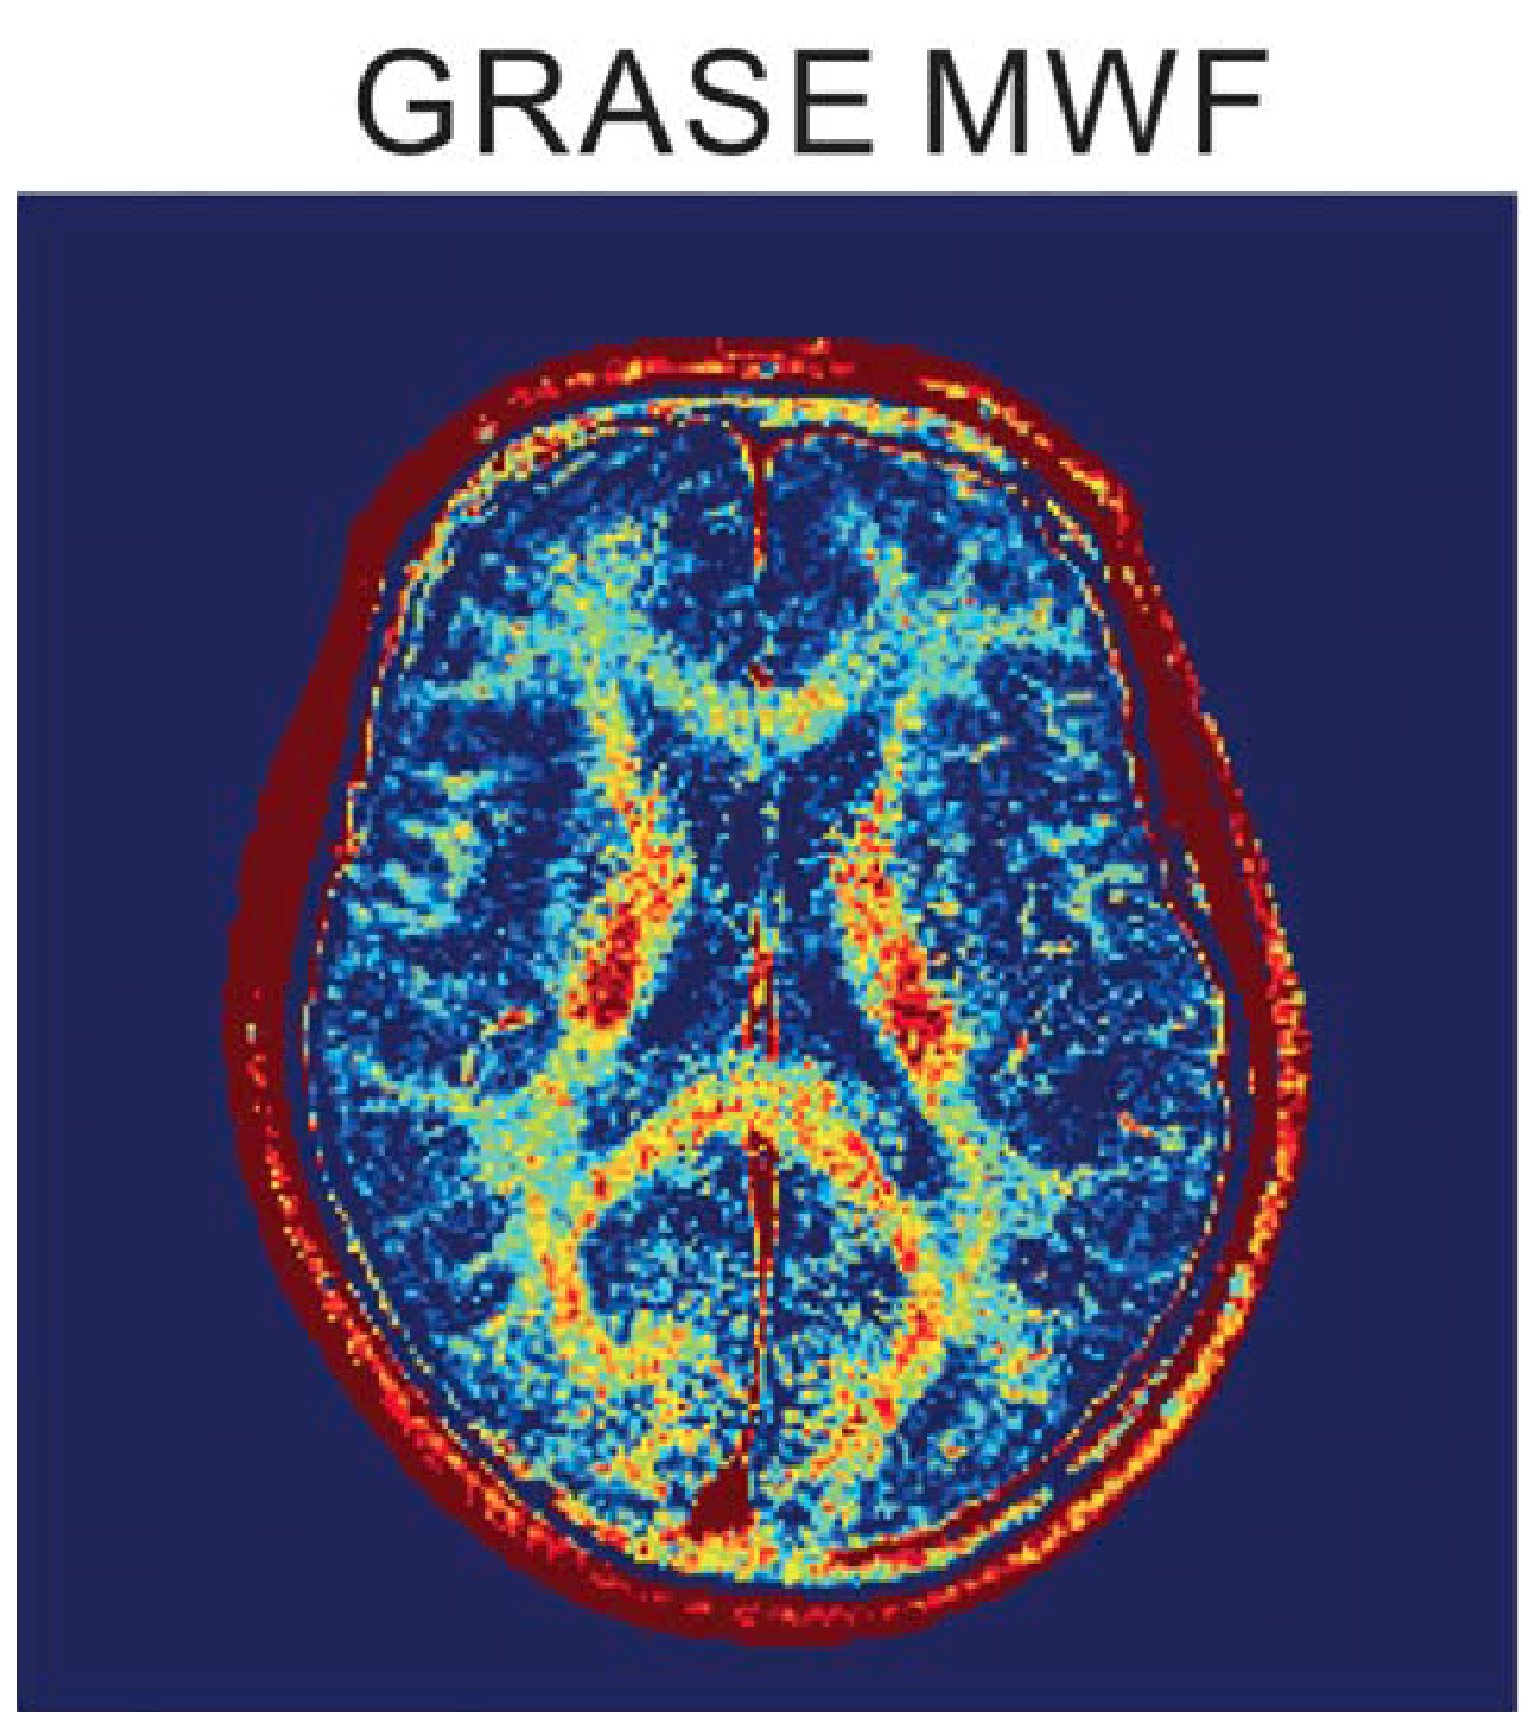
\includegraphics [height=3.8cm] {c,mwf/mwf,grase}
        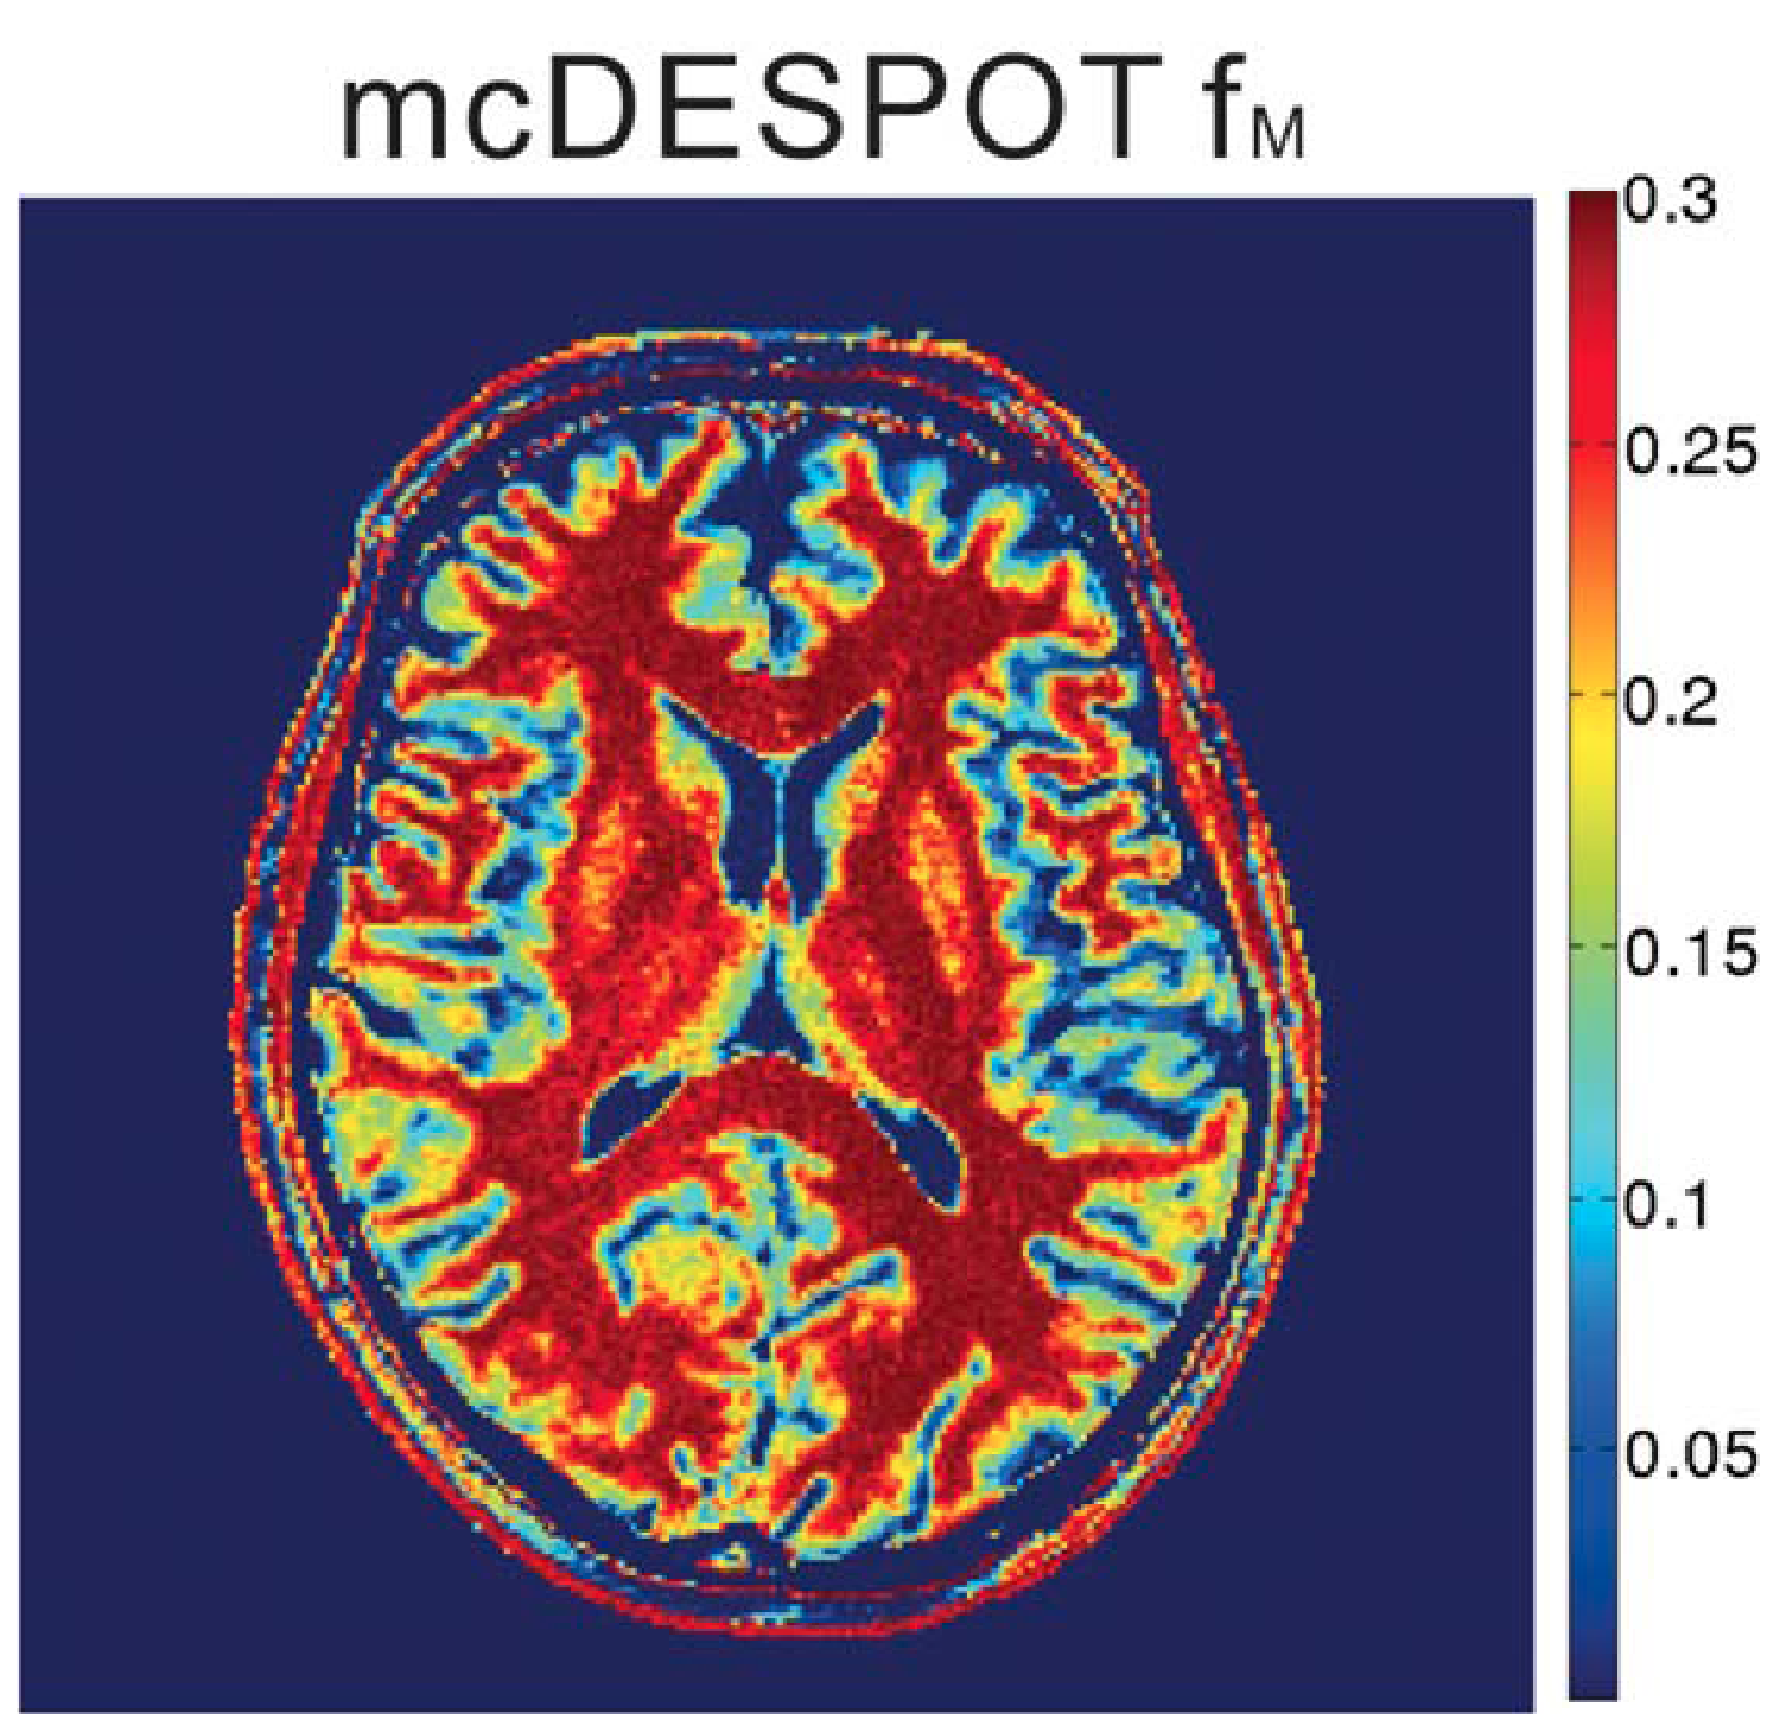
\includegraphics [height=3.8cm] {c,mwf/mwf,mcdespot}
    \end{minipage}
 	\end{figure}
\end{frame}

\begin{frame}{Summary}
	\uncover<1->{%
  	\textbf{Contributions}
  	\begin{itemize}
  		\item{Two-compartment DESS signal model}
  		\item{Fast acquisition for precise WM MWF estimation}
			\item{Proof-of-concept \invivo MWF images via KRR}
  	\end{itemize}
	}
	\uncover<2->{%
  	\textbf{Ongoing work}
  	\begin{itemize}
  		\item<2>{Systematic validation}
  		\item<3>{Further-optimized MWF acquisition}
  	\end{itemize}
	}
\end{frame}


% acknowledgment
\begin{comment}
\begin{frame}{Acknowledgments}
	\textbf{Collaborators} 
	\begin{figure}
		\centering
		\begin{minipage}[b]{0.32\textwidth}
			\centering
			\includegraphics [width=\textwidth, trim=80 40 80 30, clip] {s,ack/jeff}%
		\end{minipage}
		\begin{minipage}[b]{0.32\textwidth}
			\centering
			\includegraphics [width=\textwidth, trim=80 40 80 30, clip] {s,ack/jon}%
		\end{minipage}
		\begin{minipage}[b]{0.32\textwidth}
			\centering
			\includegraphics [width=\textwidth, trim=80 40 80 30, clip] {s,ack/clay}%
		\end{minipage}
	\end{figure}
	\textbf{Funding}
	\begin{itemize}
		\item{NIH P01 CA87634}
		\item{UM ``M-Cubed'' seed grant}
		\item{UM pre-doctoral fellowship}
	\end{itemize}
\end{frame}
\end{comment}

% bib
\begin{frame}[allowframebreaks]{References}
	\bibliography{%
		../bib/master,../bib/talk%
	}%
\end{frame}

\end{document}
